\documentclass[12pt]{beamer}

\usepackage[french]{babel}
\usepackage[T1]{fontenc}
\usepackage[utf8]{inputenc}
\usepackage{multicol}
    
\usepackage{verbatim}
\usepackage{xcolor}
\usepackage{pslatex}

\usetheme{Darmstadt}
%\usetheme{Dresden}
%\usetheme{JuanLesPins}

\newenvironment{code}
  {\fontfamily{prc}\selectfont}{}

\setbeamertemplate{navigation symbols}{}
\addtobeamertemplate{footline}{\hfill\insertframenumber/\inserttotalframenumber \hspace{1mm}

\vspace{1mm}}

 \usecolortheme[RGB={100, 0, 20}]{structure}

\title{Extension de GUIDO}
\subtitle{\`A la notation musicale contemporaine}
\author{Colas Decron, Dominique Fober, Camille Le Roi \\ GRAME}
\date{JIM - 21 Mai 2014}



\begin{document}


%%%%%%%%%%% TITRE %%%%%%%%%%%%%
    \frame{\titlepage
    
\begin{center} 
\includegraphics[width=2cm]{img/grame.pdf} \hspace{0.5cm} 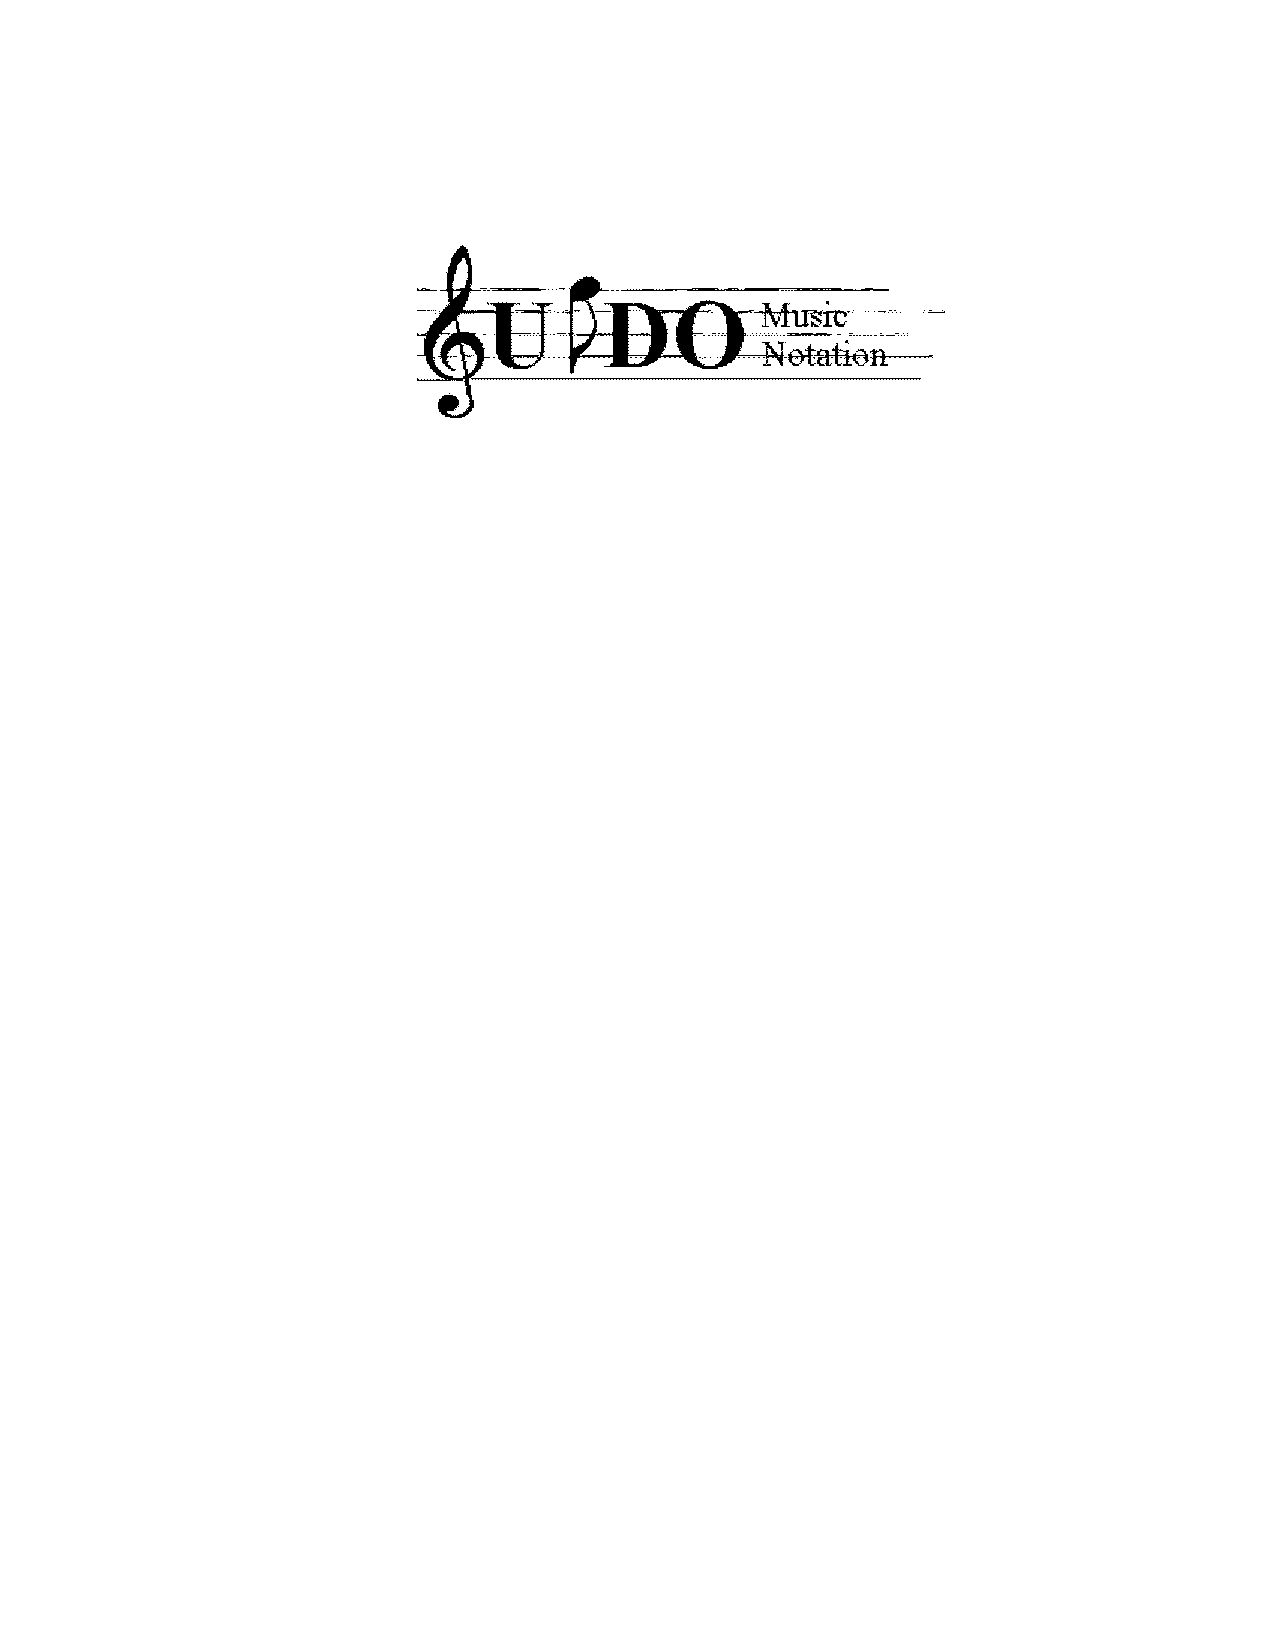
\includegraphics[width=4cm]{img/guido.pdf}\end{center}}

%%%%%%%%%% SOMMAIRE %%%%%%%%%%%    

    \begin{frame}
    \frametitle{Extension de GUIDO}
    \section{Sommaire}
    
    \Large    
    \begin{itemize}
      \item Présentation de Guido
      \begin{itemize}
        \item le langage
        \item le moteur de rendu
      \end{itemize}
      \item Nouvelles notations
      \item Améliorations du contrôle de rendu
    \end{itemize}
    
    \end{frame}

%%%%%%%%%%% GUIDO %%%%%%%%%%%%%    

% -------------------------------- Général ------------------------------
    \begin{frame}
    \frametitle{GUIDO : Description textuelle de la musique}
    \section{Guido}
    
    \large
    
    \begin{itemize}
      \item Notes : a, b, c, d, e, f, g, h
      \item Altérations : \#, \&
      \item Octave : 1 par défaut
      \item Silences : \_
      \item Durées : de la quadruple croche 1/64\\ à la ronde 1/1 ( 1/4 par défaut )
      \item Tags \begin{code} \textbackslash{}tag<paramètres>\end{code} :\\ 
      \vspace{2mm}
      \begin{code} \textbackslash{}noteFormat \textbackslash{}meter \textbackslash{}clef \textbackslash{}cresc \end{code} ...
    \end{itemize}
    
    \end{frame}
    
% -------------------------------- Paramètres ---------------------------
    \begin{frame}
    \frametitle{Contrôle de rendu}
    
    \begin{itemize}
      \item Paramètres standards :
      \begin{code}
      \begin{itemize}
        \item dx, dy
        \item size
        \item color
      \end{itemize}
      \end{code}
      \item Tags de contrôle des notes :
      \begin{code}
      \begin{itemize}
        \item \textbackslash{}noteFormat
        \item \textbackslash{}headsLeft, \textbackslash{}headsRight, \textbackslash{}headsCenter, \textbackslash{}headsNormal
        \item \textbackslash{}stemsOff, \textbackslash{}stemsAuto, \textbackslash{}stemsUp, \textbackslash{}stemsDown
      \end{itemize}
      \end{code}
    \end{itemize}
    
    \end{frame}

%%%%%%%% NOUVELLES NOTATIONS %%%%%%%    

    \begin{frame}
    \frametitle{Nouvelles notations}
    \section{Nouvelles notations}
    
    \large
    
    \begin{itemize}
      \item Micro-tonalités
      \item Glissandi
      \item Clusters
      \item Feathered Beaming
      \item Graphiques arbitraires
      \item StaffOff, staffOn
    \end{itemize}
    
    \end{frame}
    

% ---------------------------- Micro tonalités -----------------------------

    \begin{frame}
    \frametitle{Micro -Tonalités}
    \subsection{microtonalités}

    \begin{code} \textbackslash{}alter \textless{}detune\textgreater{} \end{code} \hspace{2cm} \vspace{-1cm} 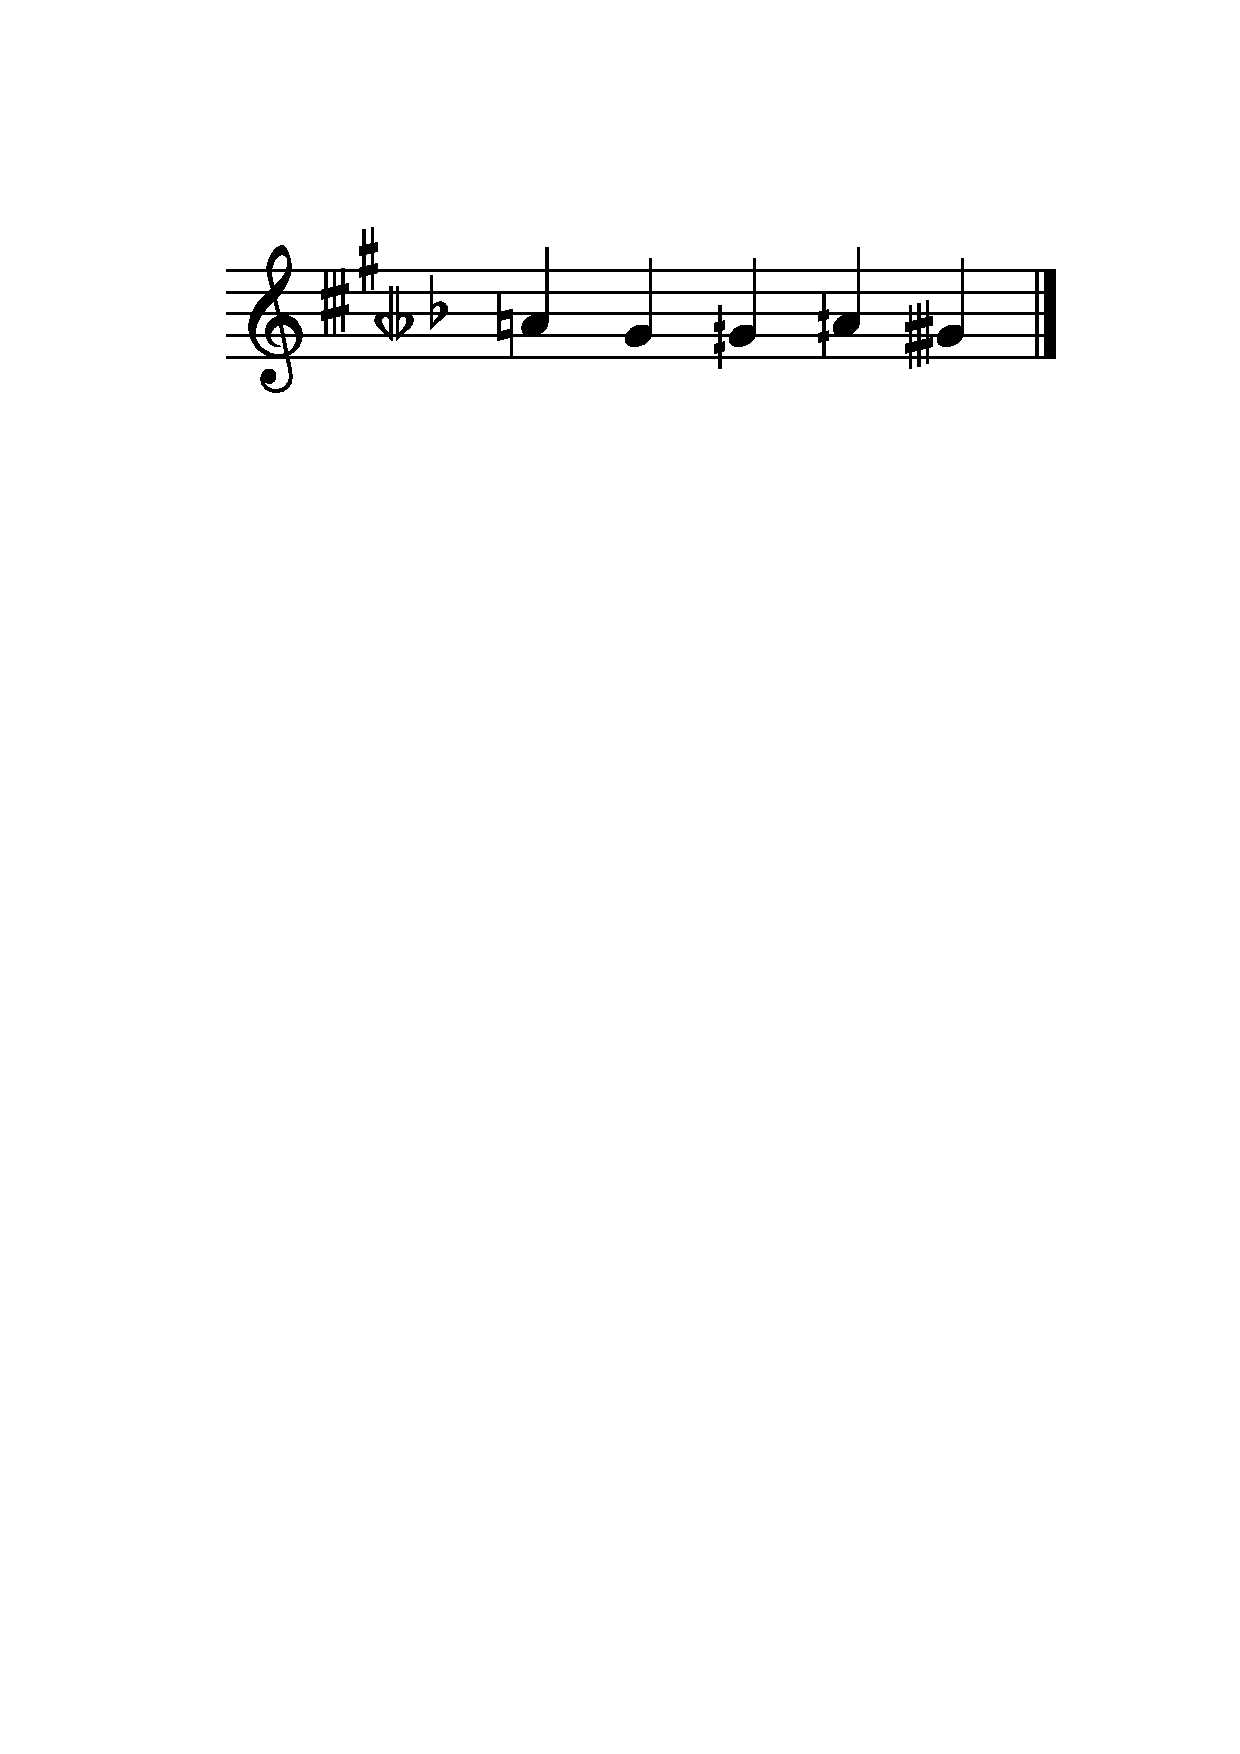
\includegraphics[width=5.3cm]{img/partitions/freekey.pdf} \\
    \begin{code} \textbackslash{}alter \textless{}detune\textgreater{} (notes) \end{code}
    
    
    \vspace{10mm}
    
    \begin{itemize}
      \item Range-tag optionnel : concerne certaines notes, ou toutes les suivantes
      \item Niveau graphique : limité au quart de ton
      \item Niveau langage : nombre flottant de demi-tons (arrondi au quart de ton le plus proche pour le rendu graphique)
    \end{itemize}
    
    \end{frame}
    
% ------------------------------- Glissandi ----------------------------------

    \begin{frame}
    \frametitle{Glissandi}
    \subsection{glissandi}
    
    \begin{code} \textbackslash{}glissando \textless{} params \textgreater{} (notes)\\ 
    \hspace{2mm} params :\\
      - fill = [ true | false ] : option de remplissage\\
      - thickness : épaisseur de la ligne
    \end{code}
    
    \vspace{5mm}
    
    \begin{multicols}{2}
    
    \begin{itemize}
      \item Range-tag
      \item Glissandi entre accords
      \item Option de remplissage
      \item Option d'épaisseur
      \item Réglage de position
    \end{itemize}
    
    \columnbreak
    
    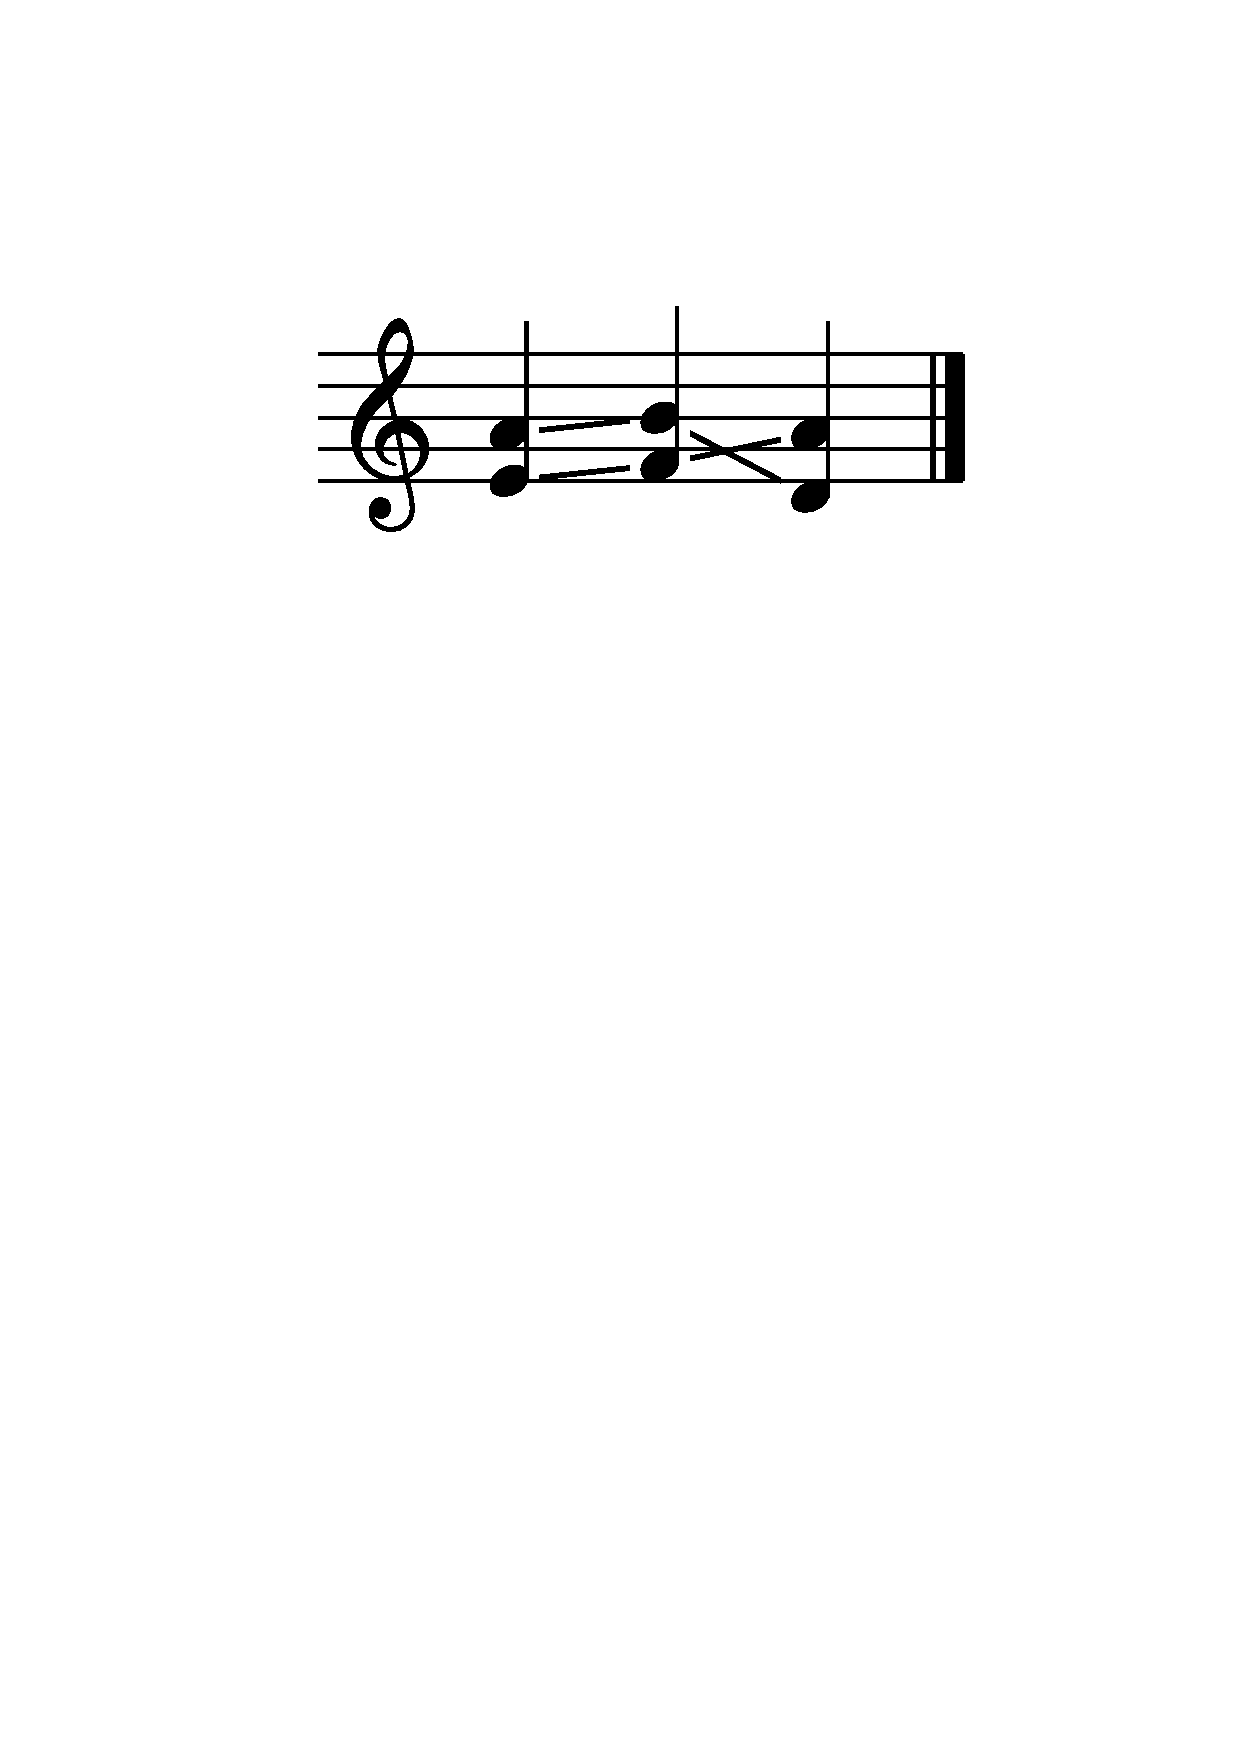
\includegraphics[width=4cm]{img/glissandosimple.pdf}
    
    \end{multicols}
    
    \end{frame}

% ---------------------------------- Clusters ----------------------------------

    \begin{frame}
    \frametitle{Clusters}
    \subsection{clusters}
    
    \begin{code} \textbackslash{}cluster \textless{} params \textgreater{} (accords) \end{code}
    
    \vspace{2mm}
    \centering  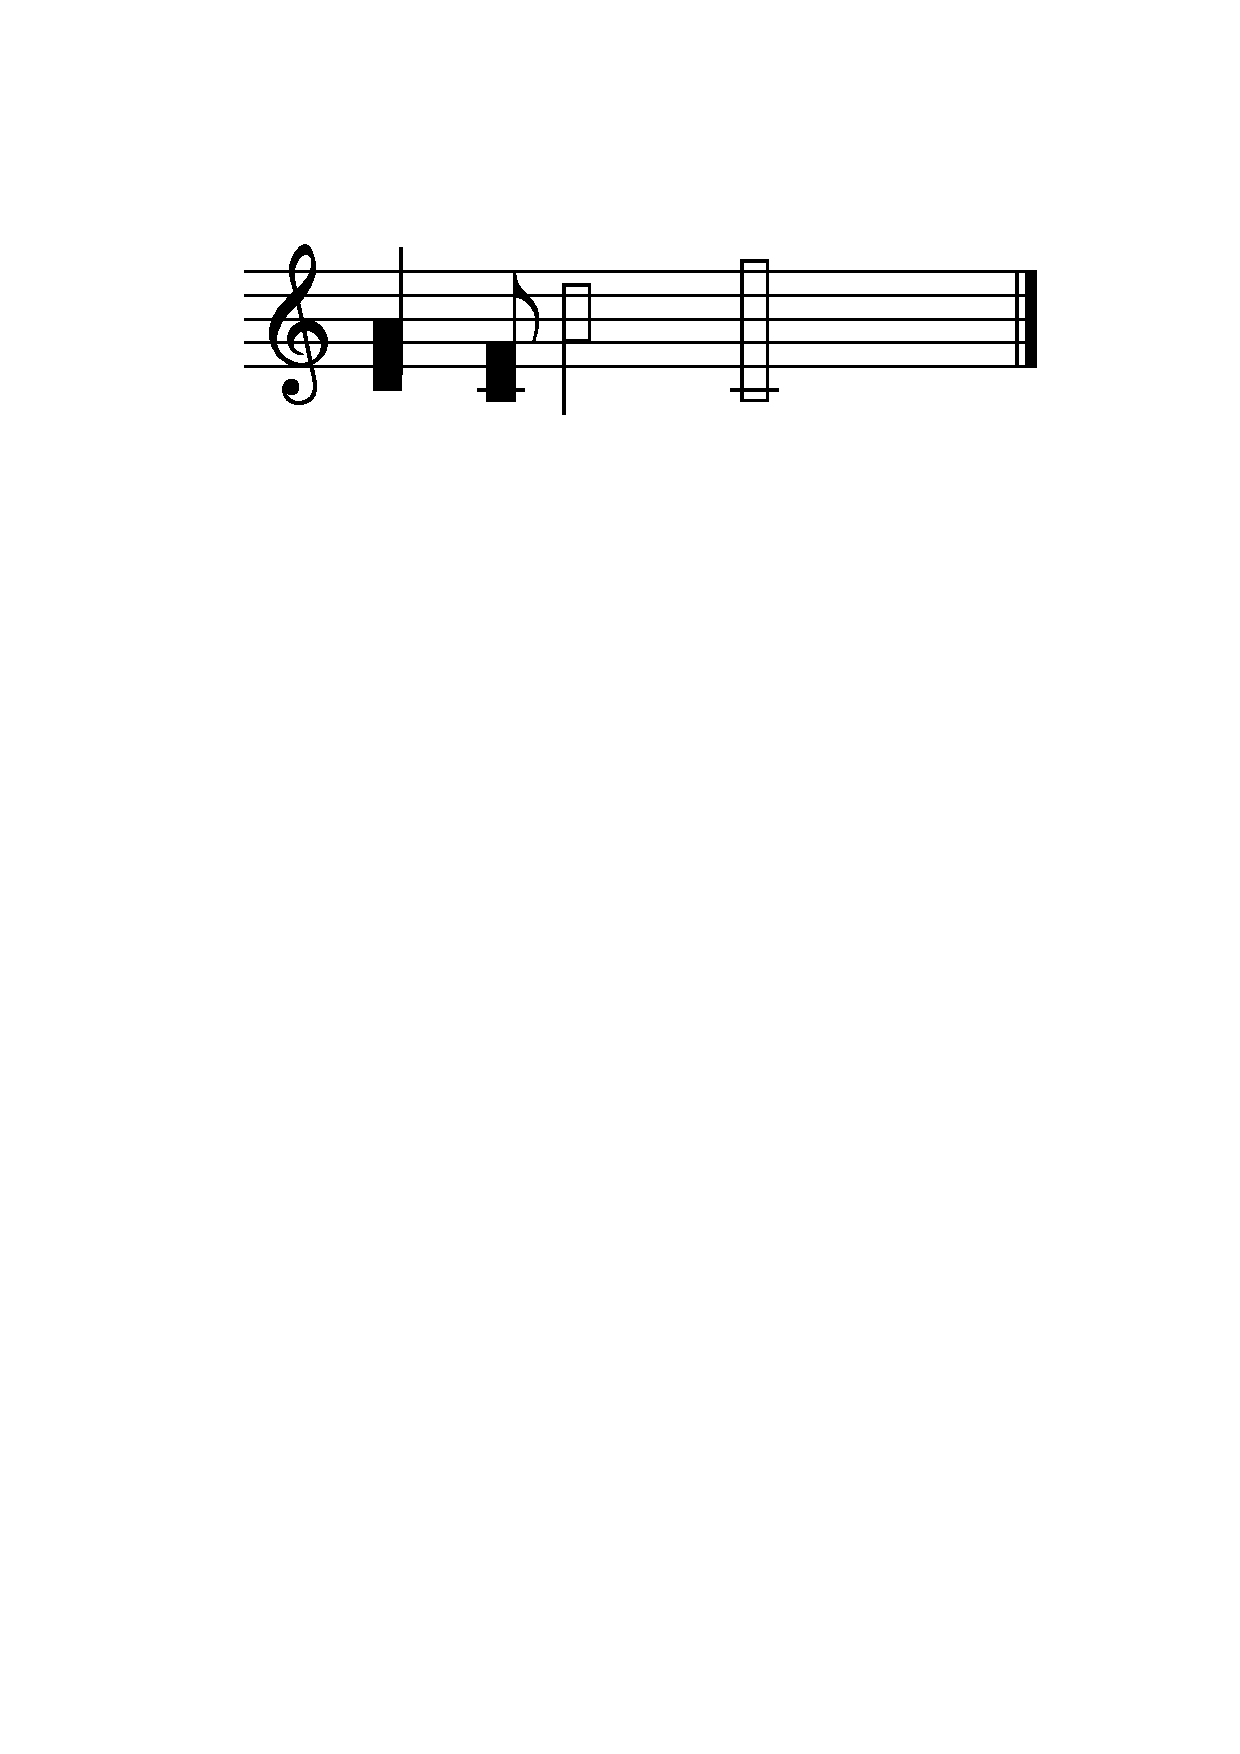
\includegraphics[width=5cm]{img/partitions/cluster.pdf}
    
    \begin{itemize}
      \item Range-tag s’appliquant \`a des accords de deux notes (les notes extr\^emes du cluster)  
      \item Remplissage et hampe suivant les mêmes règles que les accords normaux
      \item Supporte les modifications standards de format
    \end{itemize}
    
    \end{frame}

% ------------------------- Feathered Beaming ---------------------------
    \begin{frame}
    \frametitle{Feathered Beaming \small ( liens de croches en soufflet )}
    \subsection{fbeam}

    \begin{code} \textbackslash{}fBeam \textless{} params \textgreater{} (notes)\\ 
    \hspace{2mm} params :\\
      - durations = "firstDur, lastDur"\\
      - drawDuration = [ true | false ]
    \end{code}
    
    \vspace{5mm}
    
    \begin{itemize}  
      \item \textit{Accelerando} ou \textit{ritardando} exprimés à travers les liens de croches
    \end{itemize}
    
    \begin{multicols}{2}
    
    \begin{itemize}
      \item Range-tag
      \item Option \begin{code}drawDuration\end{code}
      \item Option \begin{code}durations\end{code}
      \item Chevauchement de beams
      \item Combinaisons de beams
    \end{itemize}

    \columnbreak
    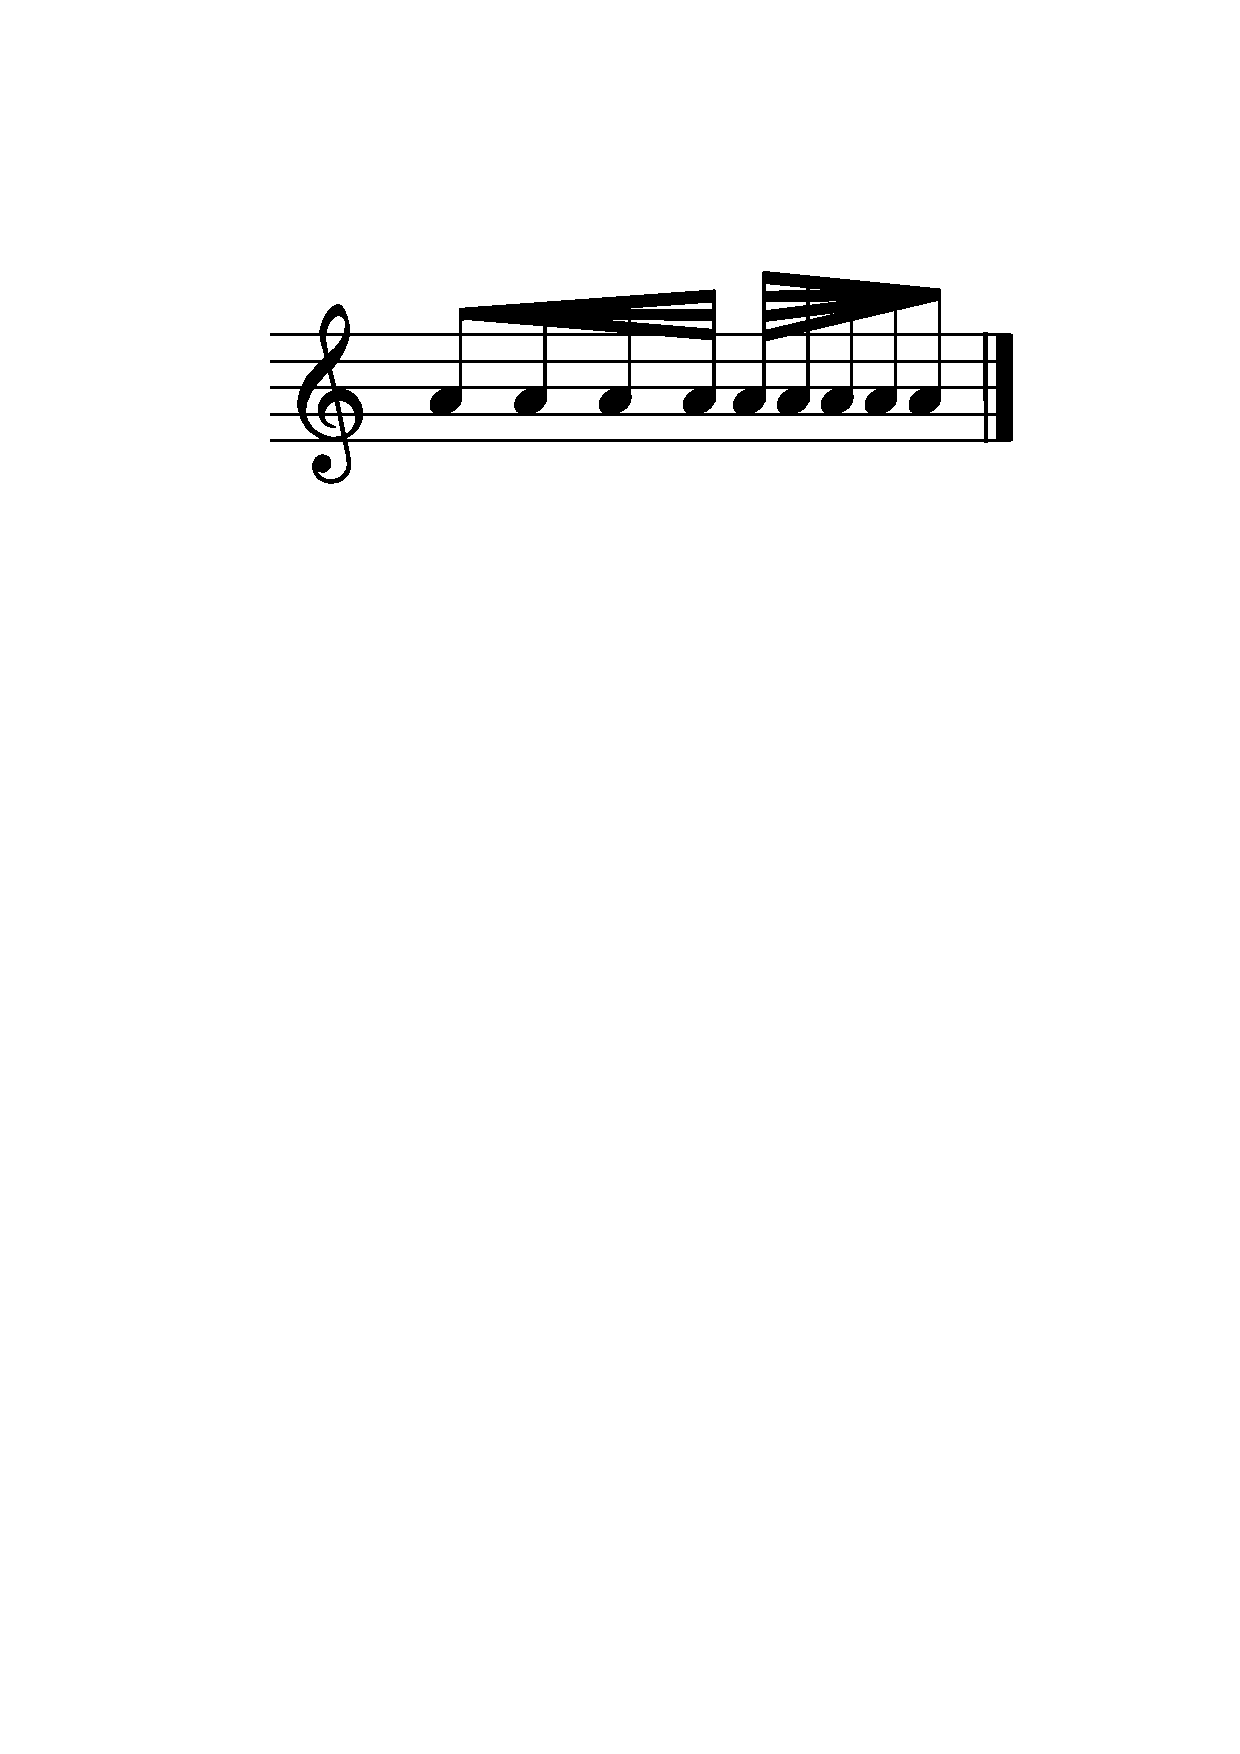
\includegraphics[width=5cm]{img/fbeamsimple.pdf}
    
    \end{multicols}
    
    \end{frame}


% ------------------------- Graphiques arbitraires --------------------------
    \begin{frame}
    \frametitle{Graphiques arbitraires}
    \subsection{graphiques}
   
    \begin{code} 
    \textbackslash{}symbol\textless{}params\textgreater{}\\
    \textbackslash{}symbol\textless{}params\textgreater{}(notes)\\
    \end{code}
    
    \begin{multicols}{2}
    
   \begin{code}
    params :\\
     - filePath : chemin du fichier\\
     - position  [ top | mid | bot ] : position de l’image
    \end{code}
    
    \columnbreak
    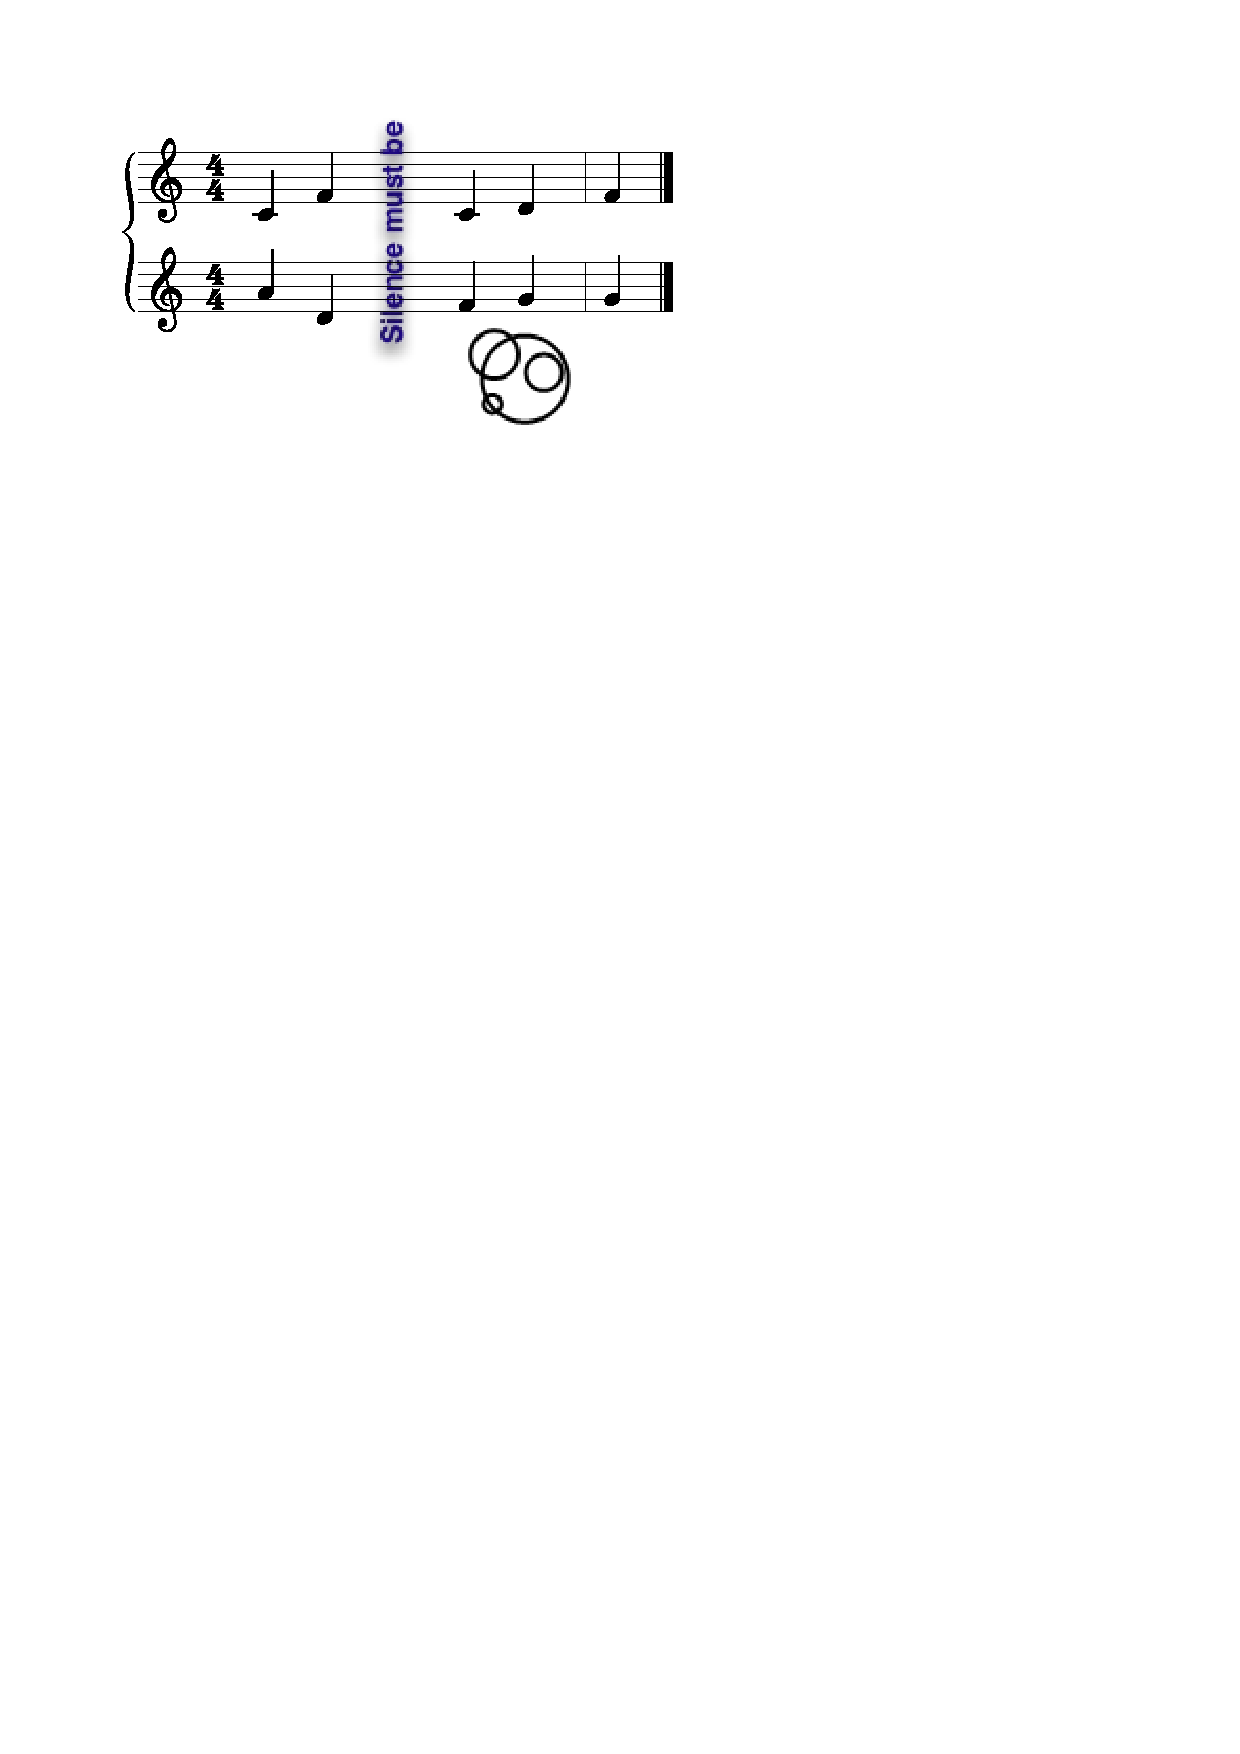
\includegraphics[width=5cm]{img/partitions/symbol.pdf}
    
    \end{multicols}
    
    \vspace{-10mm}
    \begin{itemize}
      \item Permet d'insérer une image
      \item Range-tag optionnel : \begin{itemize}
        \item l'image prend la place qu'il lui faut sur la portée
        \item l'image prend la durée des évènements entre parenthèses
      \end{itemize}
      \item Formats graphiques supportés : png, jpg ou bmp
      \item Fichier indiqué par un chemin absolu ou relatif
    \end{itemize}
    
    \end{frame}

% ----------------------------- staffOff / staffOn --------------------------------
    \begin{frame}
    \frametitle{StaffOff / staffOn}
    \subsection{staffOff}
    
    \begin{code} ... \textbackslash{}staffOff ... \hspace{1cm} \end{code} \\
    \begin{code} ... \textbackslash{}staffOn ... \end{code}
    
    \begin{center} 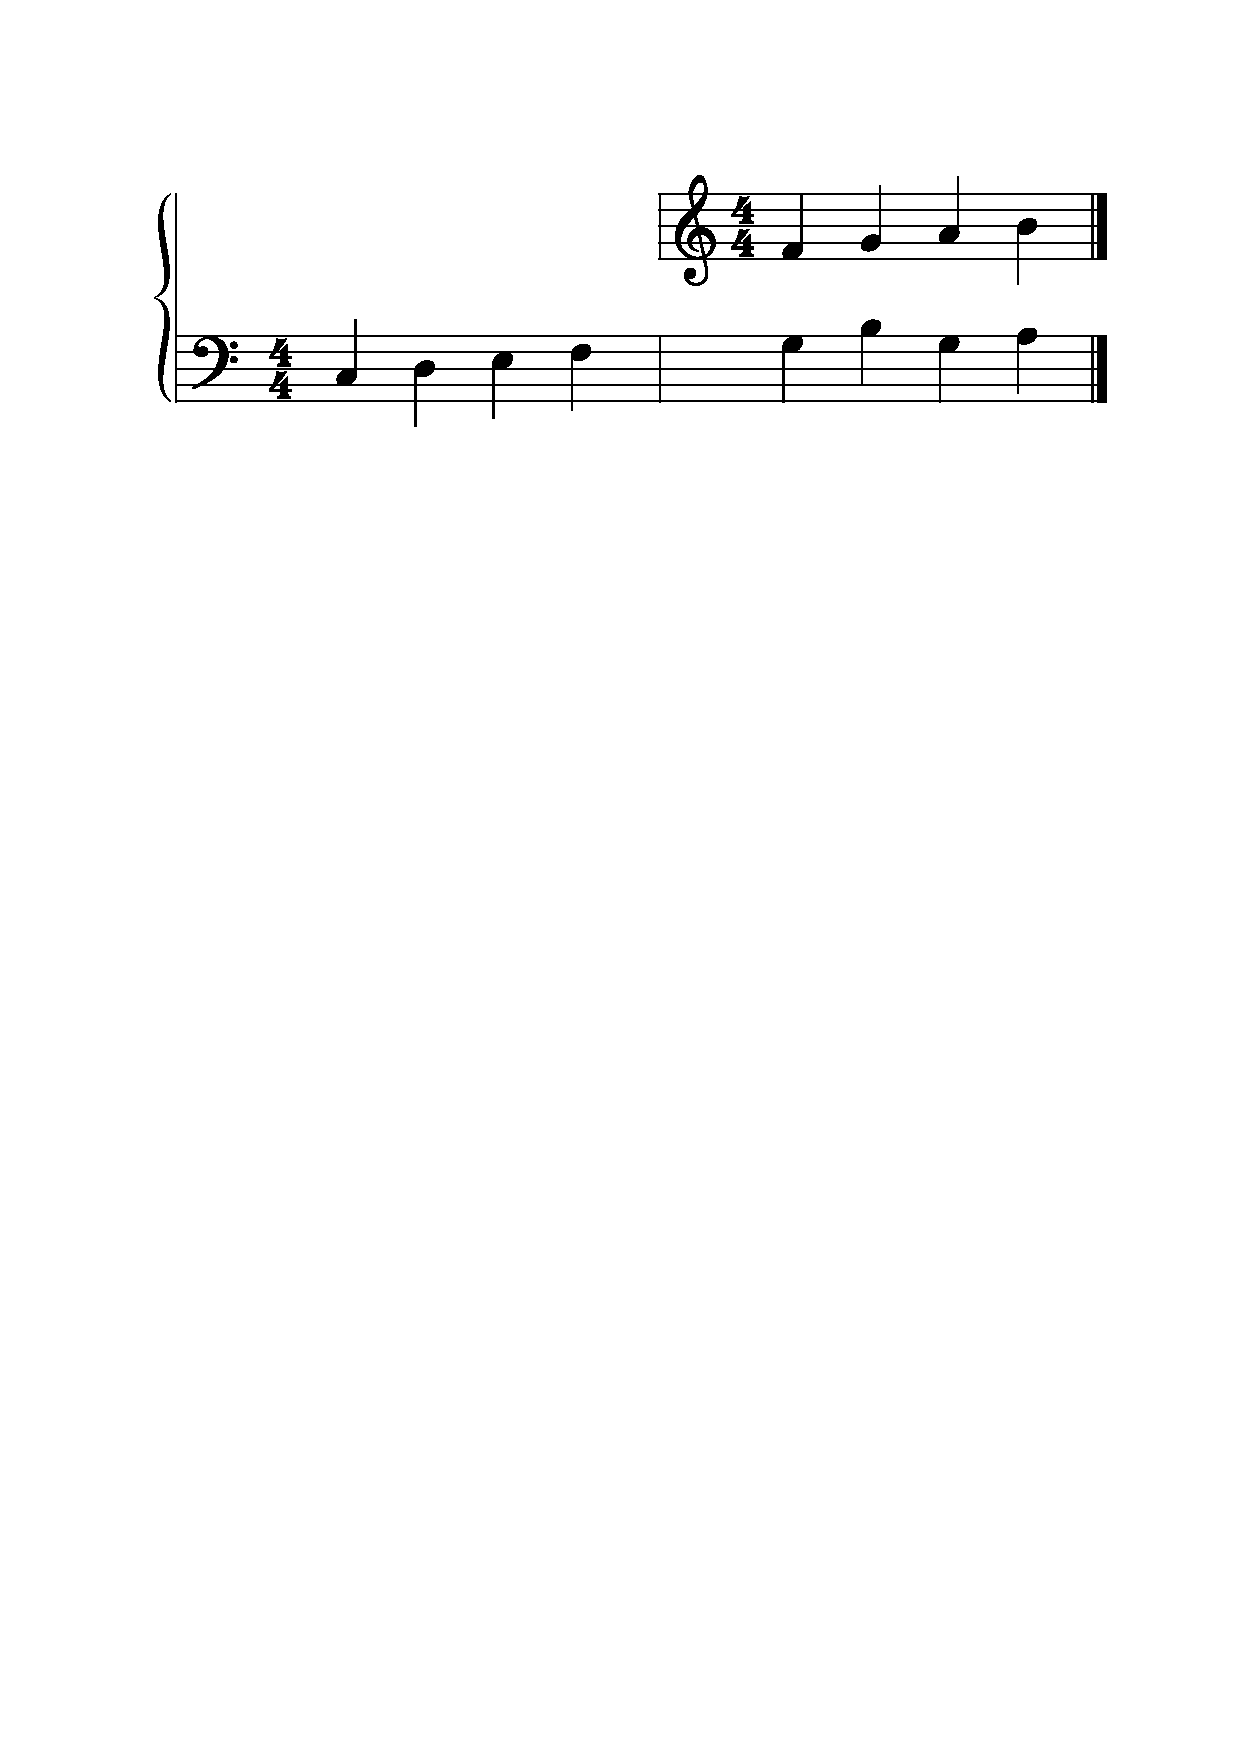
\includegraphics[width=7cm]{img/staffoff.pdf} \end{center}
    
    \vspace{-0.5cm}
    
    \begin{itemize}
      \item Permet de faire apparaître et disparaître des parties de la partition
      \item Respecte strictement l'ordre de la description textuelle (même pour les éléments simultanés)
    \end{itemize}
    
    \end{frame}
    
    
    \begin{frame}
        \frametitle{Démo}
        \subsection{demo}
        
        \begin{itemize}
        	\item Glissandi
        	\item Feathered beaming
        	\item Symbols
        \end{itemize}
        
    \end{frame}

%%%%%%%%% AMELIORATIONS DU RENDU %%%%%%%
    \begin{frame}
    \frametitle{Améliorations du rendu}
    \section{Améliorations}
    
    \large
    
    \begin{itemize}
      \item Métriques complexes
      \item Nouveaux paramètres
      \item Têtes de notes
      \item Trilles
      \item Streams
    \end{itemize}
    
    \end{frame}

% -------------------------- Métriques complexes ---------------------------
    \begin{frame}
    \frametitle{Métriques complexes}
    \subsection{metriques}
    
    \begin{itemize}
    \item Permet d’indiquer une métrique sous forme de somme.
    \end{itemize}
    
    \begin{center}
    \begin{code} \textbackslash{}meter\textless{}type="n1+n2+.../d"\textgreater{} \end{code}
    
    \vspace{5mm}
    
    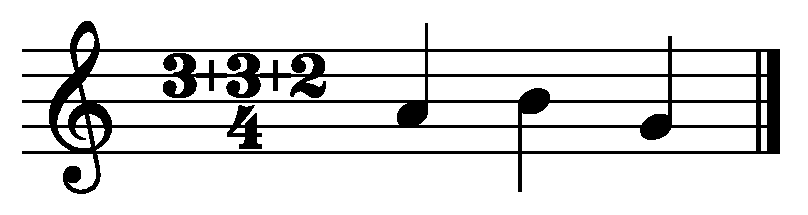
\includegraphics[width=5cm]{img/partitions/complexMeter.pdf}
    \end{center}
    
    \end{frame}
    
% -------------------------- Nouveaux paramètres ---------------------------
    \begin{frame}
    \frametitle{Nouveaux paramètres}
    \subsection{paramètres}
    
    \begin{itemize}
      \item \begin{code} \textbackslash{}staffFormat\textless{}params\textgreater{} \end{code}: épaisseur de lignes de la portée
      \item \begin{code} \textbackslash{}tuplet\textless{}params\textgreater{} \end{code}: épaisseur des lignes, taille du texte
      \item \begin{code} \textbackslash{}crescendo(notes) \textbackslash{}decrescendo(notes) \end{code}: position, épaisseur, couleur...
    \end{itemize}
    
    \vspace{2mm}
    \begin{center}
    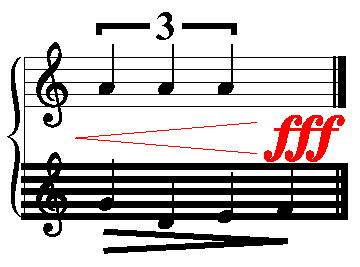
\includegraphics[width=4cm]{img/partitions/nouveauxParams.pdf}
    \end{center}
    
    \end{frame}

% --------------------------------- Têtes de notes ----------------------------------
    \begin{frame}
    \frametitle{Têtes de notes}
    \subsection{tetesnotes}
    
    \begin{code} \textbackslash{}noteFormat \textless{} style = noteHeadStyle \textgreater{}\\ 
    \textbackslash{}noteFormat \textless{} style = noteHeadStyle \textgreater{} (notes)\\ 
    \end{code}
    
    \begin{multicols}{2}

    \begin{code}
    noteHeadStyle :\\
      - x\\
      - diamond\\
      - round \\
      - square\\
      - triangle\\
      - reversedTriangle
    \end{code}
    
    \columnbreak

    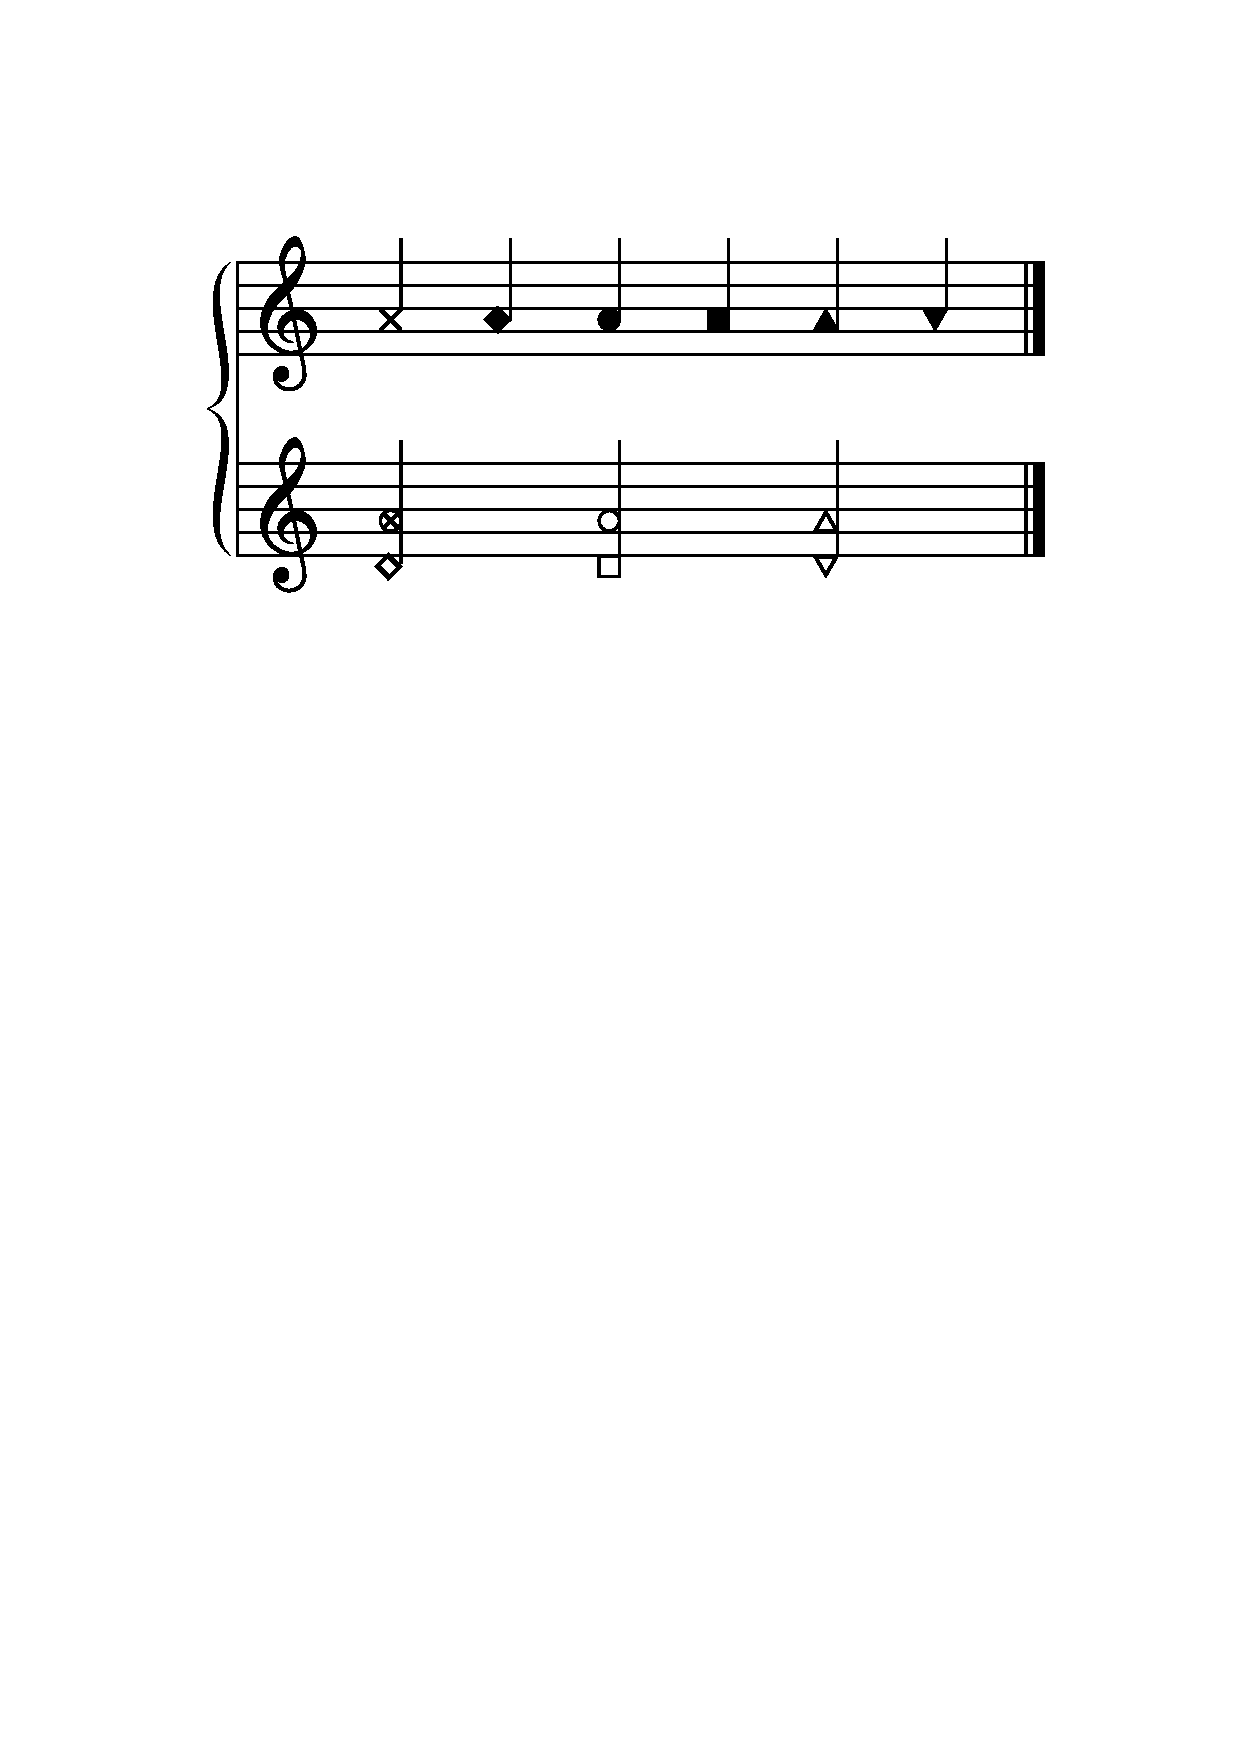
\includegraphics[width=5cm]{img/partitions/noteheads.pdf}
    
   \end{multicols}

    \begin{itemize}
      \item Range-tag optionnel
    \end{itemize}
   
    
    \end{frame}

% ------------------------------------ Trilles -----------------------------------------
    \begin{frame}
    \frametitle{Trilles}
    \subsection{trilles}
    
    \begin{center} 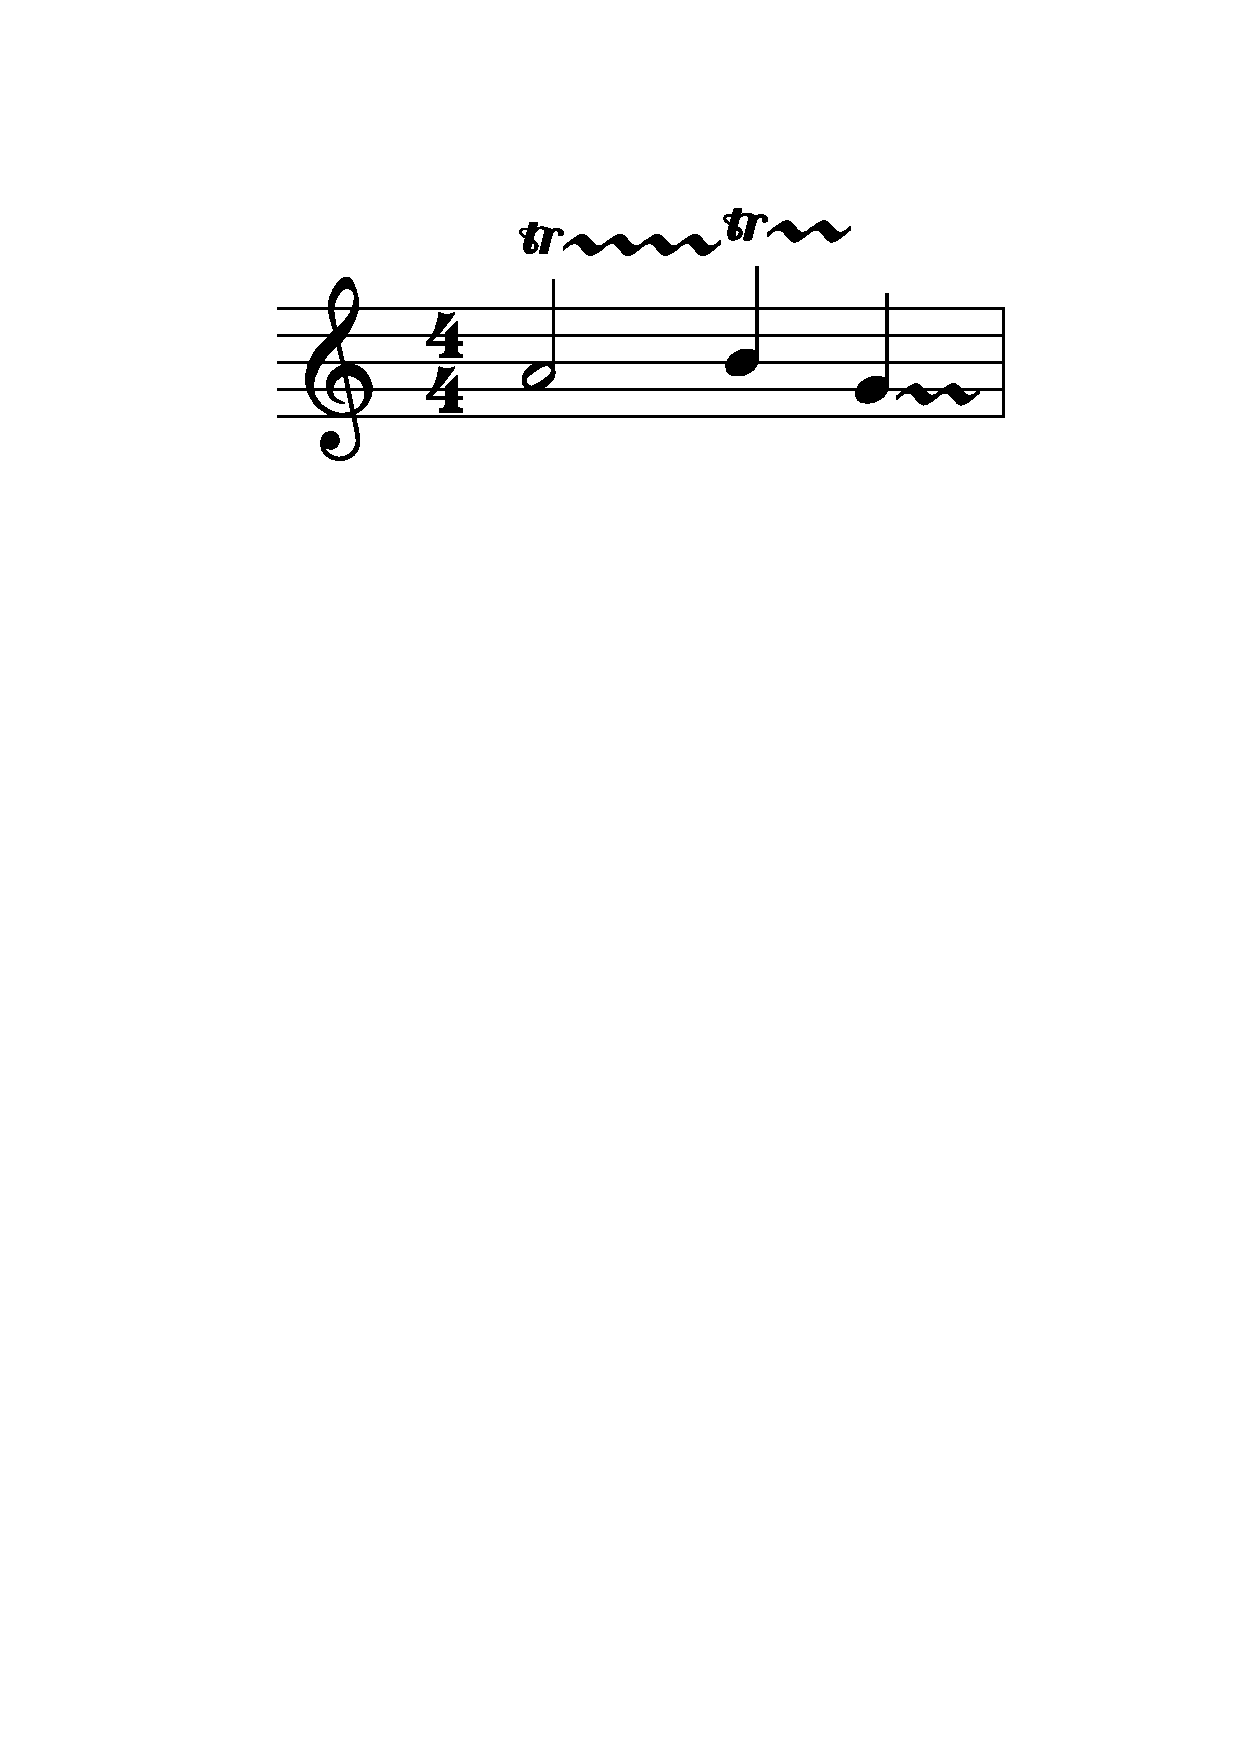
\includegraphics[width=4cm]{img/trill2.pdf} \end{center}
    
    \begin{code} \textbackslash{}trill \textless{} params \textgreater{} (accords)\\ 
    \hspace{2mm} params :\\
      - tr = [ true | false ]\\
      - anchor  = [ note | tr ]
    \end{code}
    
    \vspace{5mm}
    
    \begin{itemize}
      \item Ajout de la ligne ondulée correspondant à la durée du trille
      \item Possibilité de dessiner ou non le \textbf{tr}
      \item Possibilité d'ancrer la ligne à la tête de la note
    \end{itemize}
    
    \end{frame}

% -------------------------------------- Streaming -------------------------------------
    \begin{frame}
    \frametitle{Streaming}
    \subsection{streaming}
    
    Streaming d’une description textuelle d’une partition : 
    \begin{itemize}
      \item \begin{code} \{ [ \textbackslash{}meter\textless{}“4/4”\textgreater{} \end{code}
      \item \begin{code} a g/8 f b/4 \end{code}
      \item \begin{code} \textbackslash{}slur( f d e \end{code}
      \item \begin{code} f c) \end{code}
      \item ...
      \item \begin{code} ] \} \end{code}
    \end{itemize}
   
    \end{frame}

%%%%%%%%%%%%%%% CONCLUSION %%%%%%%%%%%%

% -------------------------------------- Applications -------------------------------------
    \begin{frame}
    \frametitle{Applications}
    \section{Conclusion}
    
    \centering
    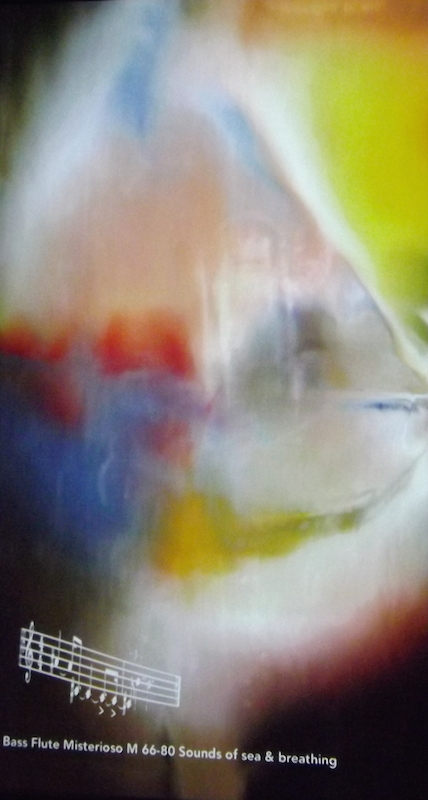
\includegraphics[width=4cm]{img/miroirs-distants.jpg}
    
    \end{frame}

% -------------------------------------- Conclusion -------------------------------------
    \begin{frame}
    \frametitle{Conclusion}
    
    
    \Large
    \begin{itemize}
      \item Embarquable
      \item Temps réel
      \item \`A venir : rendu proportionnel
    \end{itemize}
    
    \end{frame}

% -------------------------------------- Merci -------------------------------------
    \begin{frame}
    \frametitle{Merci}

    \Huge
    \begin{center}
    Merci de votre attention !
    
    \end{center}
    \end{frame}
    
    

\end{document}